\section{Biological Nanopores}

Biological nanopores are small perforations in a bilipid membrane, created
by a pore forming protein.  The majority of these proteins are toxins produced by
pathogenic bacteria, as means of killing targeted cells. They work by perforating the
cell membrane of a cell, causing cell depolarization and inducing osmotic effect. This
proces often times kills the respective cell by disrupting vital functions or spilling
its nutrients into the environment.\\

The reason scientist are intersted in studying nanopores is related to their size.
These protein structures are generally only a few nanometers in size, making them
comparable to the tiny transistors found in modern computers. Working at these small
scales has the unavoilible complication that it becomes difficult to retrieve information
from these processes. Developping sensors to probe these exotic lenghtscale is thereby
very relevant. Using ingenious methods, this is exact problem nanopores provide an
solution to, spectroscopy at the smallest scale.\\

Before delving into one of the primary application of these nanopore, Ionic current
specspectroscopy, first a brief overview will be given of the structural properties of
two popular biological nanopores.

\subsection{$\alpha$-Hemolysin ($\alpha$ HL)}

The $\alpha$-Hemolysin ($\alpha$ HL) protein is the most commonly used of pore forming
protein to create biological nanopores. It is produced by the Staphylococcus aureus, a
bacterium commonly found in the bodies microbiota.\\

The $\alpha$ HL pore(PDBID:...) is an olgimeric complex with multiple naturally occurring
variations, the most typical configuration
is a heptameric structure meaning that there are seven protomers found in the complex.
The secondary structure elements consist principally of beta-sheets, making it a member
of the Beta-barrel pore-forming toxins. Through both electrostatic and hydrophobic
interactions the $\alpha$ HL are bounded to the membrane of a target cell. Here the
monomers assemble to a 'prepore' complex that transitions to the stable pore complex by
inserting the Beta-barrel into the membrane.\\

Structurally the shape of $\alpha$ HL resembles that of a hollow mushroom. The total
hight of the complex is 11 nm and the max width is measured to be 10nm. The internal
chamber of the pore located at the cis side of the membrane membrane is called the lumen.
The lumen of $\alpha$ HL is quite constricted measuring a diameter of 3 nm. At the
membrane the lumen transitions into a protein stem refered to as the constriction of the
pore, further reducing the diameter of the chamber to a min of 1.5nm. Over the inside
surface of  $\alpha$ HL the charges are relatively uniformly distributed, this will play
an important role in further applications.\\

\todo{However, due to the slight excess of positive charges at the cis entry and the
constriction, wild-type αHL pores are found to be somewhat anion selective}

\begin{figure}[h!]
  \centering
  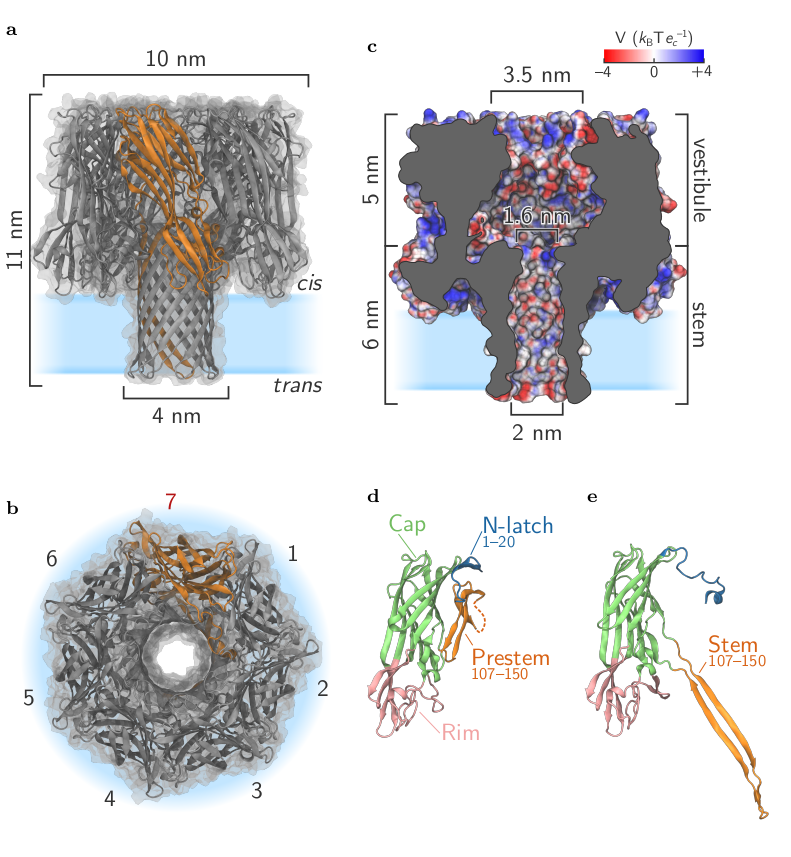
\includegraphics[width=0.5\linewidth]{Figures/alpha-hemolysin.png}
  \caption{write caption}
  \label{adsf}
\end{figure}


\subsection{Cytolysin A (ClyA)}

The Cytolysin A (ClyA) is a larger type of pore forming protein, first found to be
secreted by E. coli strains. The larger size of its lumen allows for different types of
applications compared to smaller complexes like $\alpha$ HL. Most relevant for thesis is
the fact that the larger diameter of the pores stems allows for translocation of double
stranded DNA.\\

The ClyA pore (PDBID:6MRT[cite]) is an olgimeric complex with multiple naturally
occurring variations, the most typical configuration is a dodecameric meaning that there
are twelve protomers found in the complex. The secondary structure elements consist
principally of alpha-helices, making it a member of the alpha-pore-forming toxins. The
protein formation is induced by the hydrophobic interactions between the $\beta$-hairpin
and the solvent. The main structural rearangement in this process consists of swinging
out this $\beta$-tongue and inserting it into the membrane. After this transitions the
membrane-bounded monomers oligomerize to from the final pore structure.
\todo{beter maken}

Structurally the shape of ClyA resembles that of two hollow cylinders stacked on top on
each other. This cylinder approximation will be important later on in the thesis, it will
be used to create a simplified model of the nanopore. The total hight of the complex is
14 nm and the max width is measured to be 11nm. The lumen's size of this nanopore
differentiates it from the previously discussed $\alpha$ HL. The cis entrance of the
lumen measures 6nm, while the constricted side of the pore still 3.6nm in diameter. In
contrary to the $\alpha$-HL, the inside surface of ClyA has a net negative charge
making it cation sensitive. In context of this excess charge will induce an important
 coulomb interaction between the pore and a DNA double helix, which is also negatively
 charged.


\begin{figure}[h!]
  \centering
  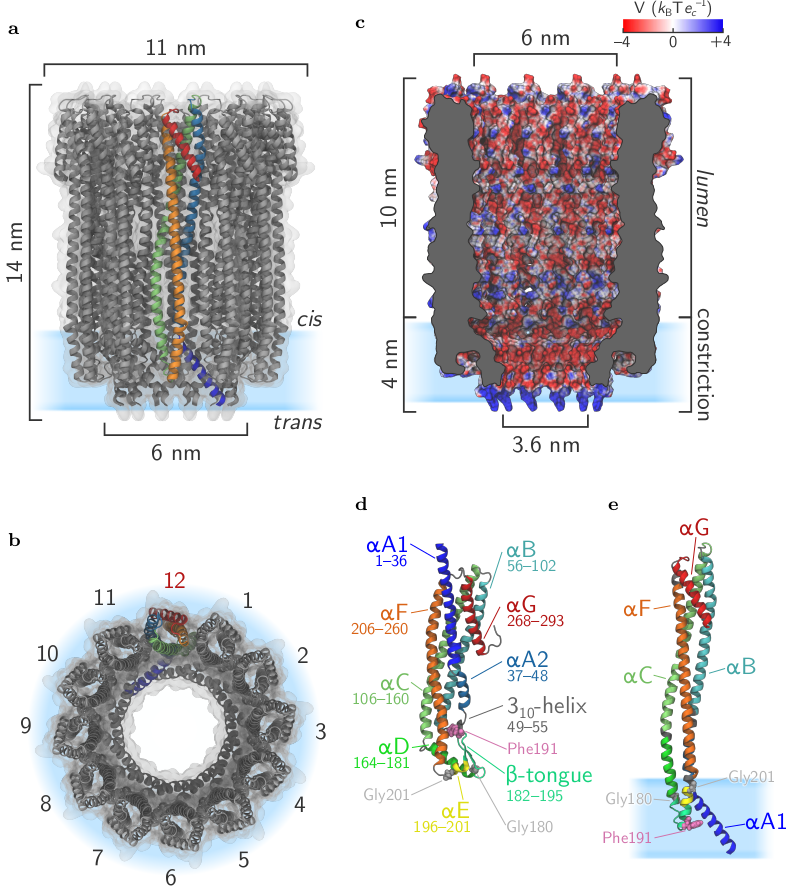
\includegraphics[width=0.5\linewidth]{Figures/cytolysinA.png}
  \caption{write caption}
  \label{adassf}
\end{figure}

\subsection{Ionic current spectroscopy}
In recent years the study of nanopores became a popular research domain, mainly
due to the development of the nanopore-based ionic current spectroscopy. For the case of
biological nanopores, this method depicted in figure .., a bilipid membrane is perforated
using a pore forming protein like $\alpha$- HL. The membrane separates two chambers of
a basin filled with a saline solution. When a potential difference is created over
the membrane, the nanopore mediates an ion current between the two sides of the basin.

This ion current through the pore can accurately be measured, if the pore is empty the
measured current is called the open pore current. However the applied ellectric field
also induces forces upon analytes dissolved in the basin. The net result of these
interactions is a flux of analytes towards and in some cases through the nanopore.
Analytes located inside of the nanopore partially block the ion current through te pore,
reducing the over measured current. Using Machine learning algorithms the timeseries of
these current fluctuation can be measured and identified with particular analytes in the
basin. This is so precise that it allows for single cell spectroscopy.

It should be noted that besides these biological nanopores, there are also inorganic
nanopores under development. An example are solid state nanopores, created by making
perforations in a semi-conductor wafer. While currently not as accessible as biological
nanopres, mainly due to their high production cost, this method has some major
advantages. First of all the material properties of provide a chemical robustness not
present in biological nanopores. The production process also allows for easy scalability
and customisability. While thus currently not as widely used as biological nanopores, due
to their customisability and robustness solid state nanopores will prove to be a
important asset in future nanotechnology.
